\documentclass[a4paper,12pt,landscape,twocolumn]{article}

\usepackage{préambule}
\usepackage{clipboard}

\geometry{left=1cm}
\setlength{\columnsep}{0.8cm}

\TitreDActivite{Créer des diagrammes}

\renewcommand{\arraystretch}{1.2}

\begin{document}

\Copy{Batons}{
	\maketitle

	On a lancé un dé à 6 faces plusieurs fois, et voici les résultats obtenus :

	\begin{center}
		\begin{tabular}{|l|c|c|c|c|c|c|}
			\hline
			Chiffre              & 1 & 2 & 3 & 4 & 5 & 6
			\\ \hline
			Nombre d'apparitions & 5 & 3 & 7 & 4 & 6 & 1
			\\ \hline
		\end{tabular}
	\end{center}

	Complète le diagramme en bâtons suivant :

	\begin{center}
		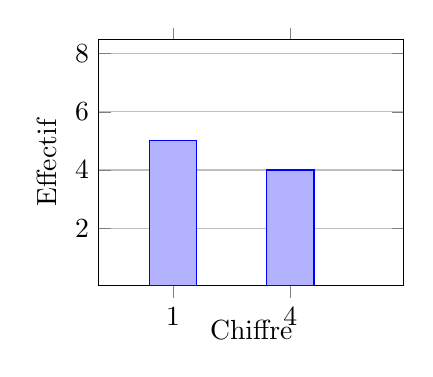
\begin{tikzpicture}
			\begin{axis}[
					width=0.45\textwidth,
					ymin=1, ymax=7.5,
					xmin=0, xmax=6,
					ybar,
					bar width=0.6cm,
					enlargelimits=0.15,
					ylabel={Effectif},
					xlabel={Chiffre},
					symbolic x coords={0, 1, 2, 3, 4, 5, 6},
					xtick=data,
					ymajorgrids = true,
					scaled y ticks = false,
					x label style={at={(axis description cs:0.5,-0.1)},anchor=north},
				]
				\addplot coordinates {
						(1,5)
						% (2,3)
						% (3,7)
						(4,4)
						% (5,6)
						% (6,1)
					};
			\end{axis}
		\end{tikzpicture}
	\end{center}
}

\newpage
\Paste{Batons}

\end{document}